\documentclass[Main.tex]{subfiles}
\begin{document}
\section{Introduction to Limits of Agreement}
\textit{\textbf{What is this from?}}
\begin{itemize}
		\item Comparing two methods of measurement is normally done by computing limits of agreement (LoA), i.e. prediction limits for
		a future difference between measurements with the two methods. When the difference is not constant it is not clear what
		this means, since the difference between the methods depends on the average; hence, unlike the case where the difference is
		constant, LoA cannot directly be translated into a prediction interval for a measurement by one method given that of another.
		\item The main point in the paper by Bland and Altman [1] is however different from the outlook in this paper; Bland and Altman
		mainly discuss whether two methods of measurement can be used interchangeably and how to assess this with the help of
		proper statistical methods to derive LoA, i.e. prediction limits for differences between two methods.
		This paper takes as starting point that the classical LoA can be converted to a prediction interval for one method given a
		measurement by the other (details in the next section). This sort of relationship can be shown in a plot as a line with slope 1
		and prediction limits as lines also with slope 1; applicable for the prediction both from method 1 to method 2 and vice versa. In
		the case of non-constant difference it would be desirable to be able to produce a similar plot, usable both ways. Thus, the aim
		of this paper is to produce a conversion from one method to another that also applies in the case where the difference between
		methods is not constant.
		\item In this paper, I set up a proper model for data for method comparison studies which in the case of constant difference between
		methods leads to the classical LoA, and in the case of linear bias gives a simple formula for the prediction. The paper only
		addresses the situation where only one measurement by each method is available, although replicate measurements by each
		method are desirable whenever possible [2]. Moreover, the situation with non-constant variance over the range of measurements
		is not covered either.
\end{itemize}
	\subsection{Limits Of Agreement}
	Bland and Altman proposed a pair of \textit{Limits of Agreement}. These
	limits are intended to demonstrate the range in which 95\% of the
	sample data should lie. The Limits of agreement centre on the
	average difference line and are 1.96 times the standard deviation
	above and below the average difference line.



	How this relates the overall population is unclear. It seems that
	it depends on an expert to decide whether or not the range of
	differences is acceptable. In a study A Bland-Altman plots compare
	two assay methods. It plots the difference between the two
	measurements on the Y axis, and the average of the two
	measurements on the X axis
	


A third element of the Bland-Altman approach, an interval known as `limits of agreement' is introduced in \citet*{BA86}
(sometimes referred to in literature as 95\% limits of agreement). Limits of agreement are used to assess whether the two methods of
measurement can be used interchangeably. \citet{BA86} refer to this as the `equivalence' of two measurement methods. The specific question to which limits of agreement are intended as the answer to must be established clearly. \citet*{BA95} comment that the limits of agreement show `how far apart measurements by the two methods were likely to be for
most individuals', a definition echoed in their 1999 paper:

\begin{quote}``We can then say that nearly all pairs
	of measurements by the two methods will be closer together than
	these extreme values, which we call 95\% limits of agreement.
	These values define the range within which most differences
	between measurements by the two methods will lie."
\end{quote}


	
	The limits of agreement (LoA) are computed by the following
	formula:
	\begin{equation}
	LoA = \bar{d} \pm 1.96 S(d)
	\end{equation}
	with $\bar{d}$ as the estimate of the inter method bias, $S(d)$ as
	the standard deviation of the differences and 1.96 is the 95\%
	quantile for the standard normal distribution. (However, in some
	literature, 2 standard deviations are used instead for
	simplicity.) 
	




The limits of agreement methodology assumes a constant level of bias throughout the range of measurements. Importantly the authors recommend prior determination of what would constitute acceptable
agreement, and that sample sizes should be predetermined to give an accurate conclusion. However \citet{mantha} highlight inadequacies in the correct application of limits of agreement, resulting in contradictory estimates of limits of agreement in various papers.

%\begin{quote}
%``How far apart measurements can be without causing difficulties
%will be a question of judgment. Ideally, it should be defined in
%advance to help in the interpretation of the method comparison and
%to choose the sample size \citep{BA86}".
%\end{quote}


For the Grubbs `F vs C' comparison, these limits
of agreement are calculated as -0.132 for the upper bound, and
-1.08 for the lower bound. Figure 1.9 shows the resultant
Bland-Altman plot, with the limits of agreement shown in dashed
lines.


	%
	%\begin{figure}[h!]
	%	\begin{center}
	%		\includegraphics[width=125mm]{GrubbsBAplot-LOA.jpeg}
	%		\caption{Bland-Altman plot with limits of agreement}\label{GrubbsBAplot-noLOA}
	%	\end{center}
	%\end{figure}
	
	The limits of agreement methodology assumes a constant level of
	bias throughout the range of measurements. As \citet*{BA86} point
	out this may not be the case. Bland and Altman advises on how to
	calculate of confidence intervals for the inter-method bias and
	the limits of agreement. Importantly the authors recommend prior
	determination of what would and would constitute acceptable
	agreement, and that sample sizes should be predetermined to give
	an accurate conclusion.
	
	\begin{quote}
		`How far apart measurements can be without causing difficulties
		will be a question of judgment. Ideally, it should be defined in
		advance to help in the interpretation of the method comparison and
		to choose the sample size.'\citep{BA86}
	\end{quote}
	
	%\subsubsection{Small Sample Sizes} The limits of agreement are
	%estimates derived from the sample studied, and will differ from
	%values relevant to the whole population, hence the importance of a
	%suitably large sample size. A different sample would give
	%different limits of agreement. Student's t-distribution is a well
	%known probability distribution used in statistical inference for
	%normally distributed populations when the sample size is small
	%\citep{student,Fisher3}. Consequently, using 't' quantiles , as
	%opposed to standard normal quantiles, may give a more appropriate
	%calculation for limits of agreement when the sample size is small.
	%For sample size $n=12$ the `t' quantile is 2.2 and the limits of
	%agreement are (-0.074,-1.143).

	
	%At least 100 historical
	%values must be used to determine the acceptable value (i.e the
	%process mean) and the process standard deviation. The principle
	%that the mean and variance of a large sample of a homogeneous
	%population is a close approximation of the population's mean and
	%variance justifies this.
	
	
	
	\subsection{Problems with Limits of Agreement}
	
	Several problems have been highlighted regarding Limits of
	Agreement. One is the somewhat arbitrary manner in which they are
	constructed. While in essence a confidence interval, they are not
	constructed a such. They are designed for future values.
	\\
	The formulation is also heavily influenced by outliers. An Example
	in \citet*{BA83} demonstrates the effect of recalculating without
	a particular outlier. Refering to the VCF data set in the same
	paper, there is more than one outlier.
	
	
	
	\subsection{Limits of Agreement}
	\citet{BA86} introduces an elaboration of the plot, adding to the
	plot `limits of agreement' to the plot. These limits are based
	upon the standard deviation of the differences. The discussion
	shall be reverted to these limits of agreement in due course.

	\subsection{Limits Of Agreement}
	
	The bias is computed as the average of the difference of paired
	assays.
	
	If one method is sometimes higher, and sometimes the other method
	is higher, the average of the differences will be close to zero.
	If it is not close to zero, this indicates that the two assay
	methods are producing different results systematically.
	
	\subsection{Appropriate Use of Limits of Agreement}
	Importantly \citet{BA99} makes the following point:
	\begin{quote}These estimates are meaningful only if we can assume
		bias and variability are uniform throughout the range of
		measurement, assumptions which can be checked graphically.
	\end{quote}
	
	The import of this statement is that, should the Bland Altman
	plot indicate that these assumptions are not met, then their
	entire methodology, as posited thus far, is inappropriate for use
	in a method comparison study. Again, in the context of potential
	outlier in the Grubbs data (figure 1.2), this raises the question
	on how to correctly continue.
	
	Carstensen attends to the issue of repeated data, using the
	expression replicate to express a repeated measurement on a
	subject by the same methods. Carstensen formulates the data as
	follows Repeated measurement - Arrangement of data into groups,
	based on the series of results of each subject.
	

	

\section{Regression-based Limits of Agreement} Assuming that
there will be no curvature in the scatter-plot, the methodology
regresses the difference of methods ($d$) on the average of those
methods ($a$) with a simple intercept slope model; $\hat{d} =
b_{0}+ b_{1}a.$ Should the slope $b_{1}$ be found to be
negligible, $\hat{d}$ takes the value $\bar{d}$.

The next step to take in calculating the limits is also a
regression, this time of the residuals as a function of the scale
of the measurements, expressed by the averages $a_{i}$;
$ \hat{R} = c_{0}+ c_{1}a_{i}$

With reference to absolute values following a half-normal
distribution with mean $\sigma\sqrt{\frac{2}{\pi}}$, \citet{BA99} formulate the regression based limits of agreement as
follows
\begin{equation}
\hat{d} \pm 1.96\sqrt{\frac{\pi}{2}}\hat{R} = \hat{d} \pm 2.46\hat{R}
\end{equation}

%------------------------------------------------%
\section{Limits of agreement for Carstensen's data}


\citet{bxc2008} describes the calculation of the limits of agreement (with the inter-method bias implicit) for both data sets, based on his formulation;

\[\hat{\alpha}_1 - \hat{\alpha}_2 \pm 2\sqrt{2\hat{\tau}^2 +\hat{\sigma}_1^2 +\hat{\sigma}_2^2 }.\]

For the `Fat' data set, the inter-method bias is shown to be $0.045$. The limits of agreement are $(-0.23 , 0.32)$

Carstensen demonstrates the use of the interaction term when computing the limits of agreement for the `Oximetry' data set. When the interaction term is omitted, the limits of agreement are $(-9.97, 14.81)$. Carstensen advises the inclusion of the interaction term for linked replicates, and hence the limits of agreement are recomputed as $(-12.18,17.12)$.



\section{Limits of Agreement}
% introduces




\begin{figure}[h!]
	\begin{center}
		\includegraphics[width=125mm]{images/GrubbsBAplot-LOA.jpeg}
		\caption{Bland-Altman plot with limits of agreement}\label{GrubbsBAplot-noLOA}
	\end{center}
\end{figure}

%But as \citet*{BA86} point out this may not be the case. Variants of the limits of agreement that overcome this
% problem shall be introduced in due course.

\subsubsection{Precision of Limits of Agreement}
The limits of agreement are estimates derived from the sample
studied, and will differ from values relevant to the whole
population. A different sample would give different limits of
agreement. \citet*{BA86} advance a formulation for confidence
intervals of the inter-method bias and the limits of agreement.
These calculations employ quantiles of the `t' distribution with
$n -1$ degrees of freedom.

%This page also shows the standard deviation (SD) of the
%differences between the two assay methods. The SD value is used to
%calculate the limits of agreement, computed as the mean bias plus
%or minus 1.96 times its SD.
%----------------------------------------------------------------------------%

\subsection{Inferences on Bland-Altman estimates}
\citet*{BA99} advises on how to calculate confidence intervals for the inter-method bias and limits of agreement.
For the inter-method bias, the confidence interval is a simply that of a mean: $\bar{d} \pm t_{(\alpha/2,n-1)} S_{d}/\sqrt{n}$.
The confidence
intervals and standard error for the limits of agreement follow from the variance of the limits of agreement, which is shown to be

\[
\mbox{Var}(LoA) = (\frac{1}{n}+\frac{1.96^{2}}{2(n-1)})s_{d}^{2}.
\]

If $n$ is sufficiently large this can be following approximation
can be used
\[
\mbox{Var}(LoA) \approx 1.71^{2}\frac{s_{d}^{2}}{n}.
\]
Consequently the standard errors of both limits can be
approximated as $1.71$ times the standard error of the
differences.

A $95\%$ confidence interval can be determined, by means of the
\emph{t} distribution with $n-1$ degrees of freedom. However, \citet*{BA99} comment that such calculations  may be `somewhat optimistic' on account of the associated assumptions not being realized.

%\subsubsection{Small Sample Sizes} The limits of agreement are
%estimates derived from the sample studied, and will differ from
%values relevant to the whole population, hence the importance of a
%suitably large sample size. A different sample would give
%different limits of agreement. Student's t-distribution is a well
%known probability distribution used in statistical inference for
%normally distributed populations when the sample size is small
%\citep{student,Fisher3}. Consequently, using 't' quantiles , as
%opposed to standard normal quantiles, may give a more appropriate
%calculation for limits of agreement when the sample size is small.
%For sample size $n=12$ the `t' quantile is 2.2 and the limits of
%agreement are (-0.074,-1.143).



\addcontentsline{toc}{section}{Bibliography}
\bibliography{DB-txfrbib}		
	

	
	


\end{document}
